% Created by tikzDevice version 0.10.1 on 2016-06-20 09:12:59
% !TEX encoding = UTF-8 Unicode
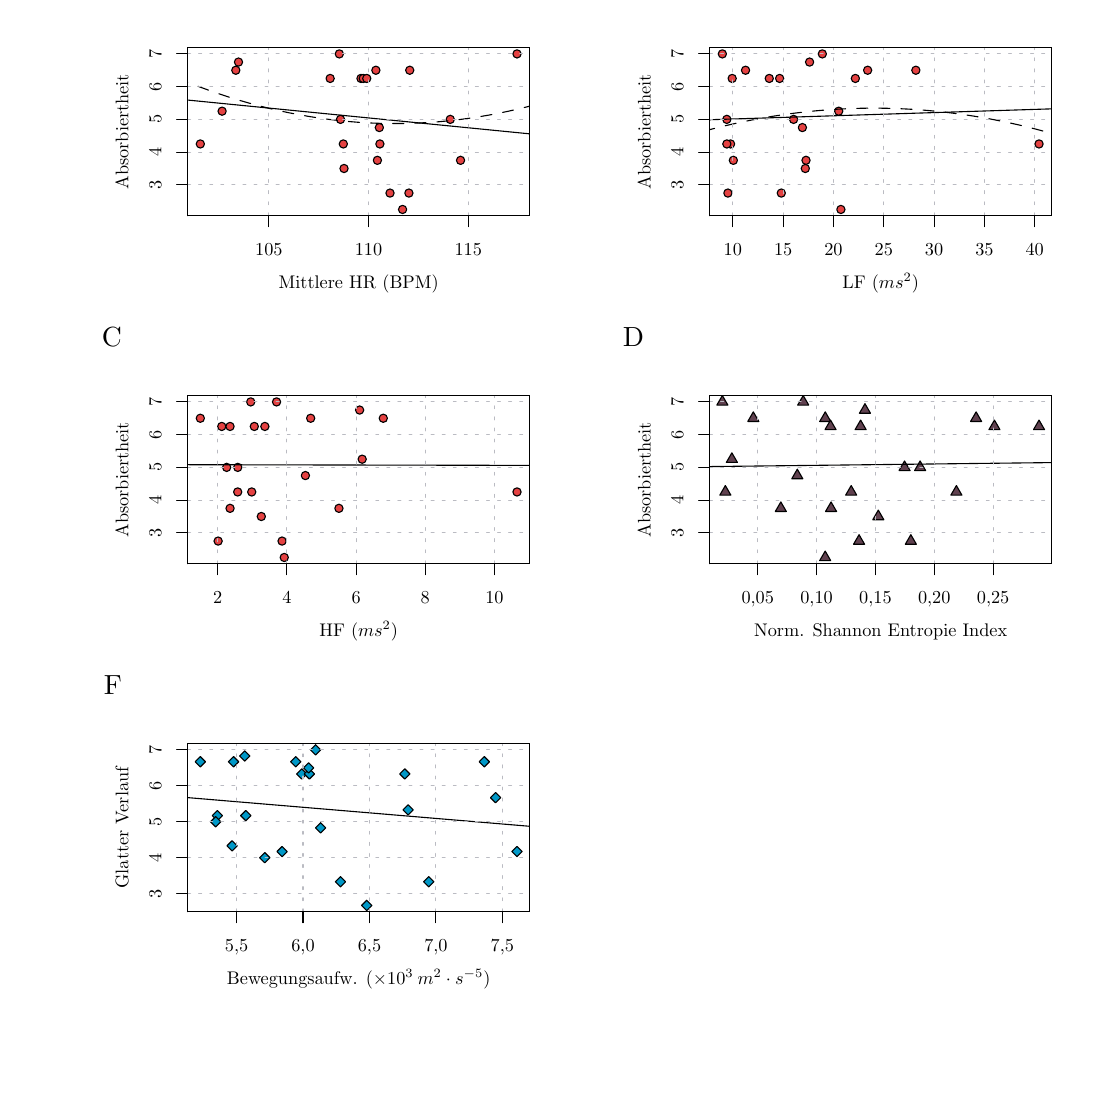
\begin{tikzpicture}[x=1pt,y=1pt]
\definecolor{fillColor}{RGB}{255,255,255}
\path[use as bounding box,fill=fillColor,fill opacity=0.00] (0,0) rectangle (377.25,377.25);
\begin{scope}
\path[clip] ( 57.82,309.32) rectangle (181.40,370.02);
\definecolor{drawColor}{RGB}{0,0,0}
\definecolor{fillColor}{RGB}{229,66,66}

\path[draw=drawColor,line width= 0.4pt,line join=round,line cap=round,fill=fillColor] (135.47,311.56) circle (  1.49);

\path[draw=drawColor,line width= 0.4pt,line join=round,line cap=round,fill=fillColor] (137.75,317.48) circle (  1.49);

\path[draw=drawColor,line width= 0.4pt,line join=round,line cap=round,fill=fillColor] (114.06,335.23) circle (  1.49);

\path[draw=drawColor,line width= 0.4pt,line join=round,line cap=round,fill=fillColor] (109.30,358.90) circle (  1.49);

\path[draw=drawColor,line width= 0.4pt,line join=round,line cap=round,fill=fillColor] (130.93,317.48) circle (  1.49);

\path[draw=drawColor,line width= 0.4pt,line join=round,line cap=round,fill=fillColor] (127.27,335.23) circle (  1.49);

\path[draw=drawColor,line width= 0.4pt,line join=round,line cap=round,fill=fillColor] (120.44,358.90) circle (  1.49);

\path[draw=drawColor,line width= 0.4pt,line join=round,line cap=round,fill=fillColor] (121.26,358.90) circle (  1.49);

\path[draw=drawColor,line width= 0.4pt,line join=round,line cap=round,fill=fillColor] (156.42,329.31) circle (  1.49);

\path[draw=drawColor,line width= 0.4pt,line join=round,line cap=round,fill=fillColor] (152.70,344.11) circle (  1.49);

\path[draw=drawColor,line width= 0.4pt,line join=round,line cap=round,fill=fillColor] (138.06,361.86) circle (  1.49);

\path[draw=drawColor,line width= 0.4pt,line join=round,line cap=round,fill=fillColor] ( 62.39,335.23) circle (  1.49);

\path[draw=drawColor,line width= 0.4pt,line join=round,line cap=round,fill=fillColor] ( 70.26,347.07) circle (  1.49);

\path[draw=drawColor,line width= 0.4pt,line join=round,line cap=round,fill=fillColor] ( 75.21,361.86) circle (  1.49);

\path[draw=drawColor,line width= 0.4pt,line join=round,line cap=round,fill=fillColor] ( 76.18,364.82) circle (  1.49);

\path[draw=drawColor,line width= 0.4pt,line join=round,line cap=round,fill=fillColor] (126.37,329.31) circle (  1.49);

\path[draw=drawColor,line width= 0.4pt,line join=round,line cap=round,fill=fillColor] (127.07,341.15) circle (  1.49);

\path[draw=drawColor,line width= 0.4pt,line join=round,line cap=round,fill=fillColor] (125.82,361.86) circle (  1.49);

\path[draw=drawColor,line width= 0.4pt,line join=round,line cap=round,fill=fillColor] (176.82,367.77) circle (  1.49);

\path[draw=drawColor,line width= 0.4pt,line join=round,line cap=round,fill=fillColor] (114.31,326.36) circle (  1.49);

\path[draw=drawColor,line width= 0.4pt,line join=round,line cap=round,fill=fillColor] (113.04,344.11) circle (  1.49);

\path[draw=drawColor,line width= 0.4pt,line join=round,line cap=round,fill=fillColor] (112.62,367.77) circle (  1.49);

\path[draw=drawColor,line width= 0.4pt,line join=round,line cap=round,fill=fillColor] (122.52,358.90) circle (  1.49);
\end{scope}
\begin{scope}
\path[clip] (  0.00,  0.00) rectangle (377.25,377.25);
\definecolor{drawColor}{RGB}{0,0,0}

\path[draw=drawColor,line width= 0.4pt,line join=round,line cap=round] ( 87.14,309.32) -- (159.21,309.32);

\path[draw=drawColor,line width= 0.4pt,line join=round,line cap=round] ( 87.14,309.32) -- ( 87.14,305.36);

\path[draw=drawColor,line width= 0.4pt,line join=round,line cap=round] (123.17,309.32) -- (123.17,305.36);

\path[draw=drawColor,line width= 0.4pt,line join=round,line cap=round] (159.21,309.32) -- (159.21,305.36);

\node[text=drawColor,anchor=base,inner sep=0pt, outer sep=0pt, scale=  0.66] at ( 87.14,295.06) {105};

\node[text=drawColor,anchor=base,inner sep=0pt, outer sep=0pt, scale=  0.66] at (123.17,295.06) {110};

\node[text=drawColor,anchor=base,inner sep=0pt, outer sep=0pt, scale=  0.66] at (159.21,295.06) {115};

\path[draw=drawColor,line width= 0.4pt,line join=round,line cap=round] ( 57.82,320.44) -- ( 57.82,367.77);

\path[draw=drawColor,line width= 0.4pt,line join=round,line cap=round] ( 57.82,320.44) -- ( 53.86,320.44);

\path[draw=drawColor,line width= 0.4pt,line join=round,line cap=round] ( 57.82,332.27) -- ( 53.86,332.27);

\path[draw=drawColor,line width= 0.4pt,line join=round,line cap=round] ( 57.82,344.11) -- ( 53.86,344.11);

\path[draw=drawColor,line width= 0.4pt,line join=round,line cap=round] ( 57.82,355.94) -- ( 53.86,355.94);

\path[draw=drawColor,line width= 0.4pt,line join=round,line cap=round] ( 57.82,367.77) -- ( 53.86,367.77);

\node[text=drawColor,rotate= 90.00,anchor=base,inner sep=0pt, outer sep=0pt, scale=  0.66] at ( 48.31,320.44) {3};

\node[text=drawColor,rotate= 90.00,anchor=base,inner sep=0pt, outer sep=0pt, scale=  0.66] at ( 48.31,332.27) {4};

\node[text=drawColor,rotate= 90.00,anchor=base,inner sep=0pt, outer sep=0pt, scale=  0.66] at ( 48.31,344.11) {5};

\node[text=drawColor,rotate= 90.00,anchor=base,inner sep=0pt, outer sep=0pt, scale=  0.66] at ( 48.31,355.94) {6};

\node[text=drawColor,rotate= 90.00,anchor=base,inner sep=0pt, outer sep=0pt, scale=  0.66] at ( 48.31,367.77) {7};

\path[draw=drawColor,line width= 0.4pt,line join=round,line cap=round] ( 57.82,309.32) --
	(181.40,309.32) --
	(181.40,370.02) --
	( 57.82,370.02) --
	( 57.82,309.32);
\end{scope}
\begin{scope}
\path[clip] (  0.00,251.50) rectangle (188.62,377.25);
\definecolor{drawColor}{RGB}{0,0,0}

\node[text=drawColor,anchor=base,inner sep=0pt, outer sep=0pt, scale=  0.66] at (119.61,283.18) {Mittlere HR (BPM)};

\node[text=drawColor,rotate= 90.00,anchor=base,inner sep=0pt, outer sep=0pt, scale=  0.66] at ( 36.43,339.67) {Absorbiertheit};
\end{scope}
\begin{scope}
\path[clip] ( 57.82,309.32) rectangle (181.40,370.02);
\definecolor{drawColor}{RGB}{0,0,0}

\path[draw=drawColor,line width= 0.4pt,line join=round,line cap=round] ( 57.82,351.09) -- (181.40,338.88);

\path[draw=drawColor,line width= 0.4pt,dash pattern=on 4pt off 4pt ,line join=round,line cap=round] ( 18.57,377.25) --
	( 18.67,377.19) --
	( 22.27,375.04) --
	( 25.88,372.96) --
	( 29.48,370.94) --
	( 33.08,369.00) --
	( 36.69,367.12) --
	( 40.29,365.32) --
	( 43.89,363.58) --
	( 47.50,361.91) --
	( 51.10,360.31) --
	( 54.70,358.78) --
	( 58.31,357.32) --
	( 61.91,355.93) --
	( 65.51,354.61) --
	( 69.12,353.35) --
	( 72.72,352.17) --
	( 76.33,351.05) --
	( 79.93,350.01) --
	( 83.53,349.03) --
	( 87.14,348.12) --
	( 90.74,347.28) --
	( 94.34,346.51) --
	( 97.95,345.81) --
	(101.55,345.18) --
	(105.15,344.61) --
	(108.76,344.12) --
	(112.36,343.70) --
	(115.96,343.34) --
	(119.57,343.05) --
	(123.17,342.83) --
	(126.78,342.69) --
	(130.38,342.61) --
	(133.98,342.60) --
	(137.59,342.65) --
	(141.19,342.78) --
	(144.79,342.98) --
	(148.40,343.24) --
	(152.00,343.58) --
	(155.60,343.98) --
	(159.21,344.46) --
	(162.81,345.00) --
	(166.41,345.61) --
	(170.02,346.29) --
	(173.62,347.04) --
	(177.23,347.86) --
	(180.83,348.74) --
	(184.43,349.70) --
	(188.04,350.72) --
	(191.64,351.82) --
	(195.24,352.98);
\definecolor{drawColor}{RGB}{186,187,194}

\path[draw=drawColor,line width= 0.4pt,dash pattern=on 1pt off 3pt ,line join=round,line cap=round] ( 87.14,309.32) -- ( 87.14,370.02);

\path[draw=drawColor,line width= 0.4pt,dash pattern=on 1pt off 3pt ,line join=round,line cap=round] (123.17,309.32) -- (123.17,370.02);

\path[draw=drawColor,line width= 0.4pt,dash pattern=on 1pt off 3pt ,line join=round,line cap=round] (159.21,309.32) -- (159.21,370.02);

\path[draw=drawColor,line width= 0.4pt,dash pattern=on 1pt off 3pt ,line join=round,line cap=round] ( 57.82,320.44) -- (181.40,320.44);

\path[draw=drawColor,line width= 0.4pt,dash pattern=on 1pt off 3pt ,line join=round,line cap=round] ( 57.82,332.27) -- (181.40,332.27);

\path[draw=drawColor,line width= 0.4pt,dash pattern=on 1pt off 3pt ,line join=round,line cap=round] ( 57.82,344.11) -- (181.40,344.11);

\path[draw=drawColor,line width= 0.4pt,dash pattern=on 1pt off 3pt ,line join=round,line cap=round] ( 57.82,355.94) -- (181.40,355.94);

\path[draw=drawColor,line width= 0.4pt,dash pattern=on 1pt off 3pt ,line join=round,line cap=round] ( 57.82,367.77) -- (181.40,367.77);
\end{scope}
\begin{scope}
\path[clip] (  0.00,  0.00) rectangle (377.25,377.25);
\definecolor{drawColor}{RGB}{0,0,0}

\path[draw=drawColor,line width= 0.4pt,line join=round,line cap=round] ( 57.82,309.32) --
	(181.40,309.32) --
	(181.40,370.02) --
	( 57.82,370.02) --
	( 57.82,309.32);
\end{scope}
\begin{scope}
\path[clip] (246.44,309.32) rectangle (370.02,370.02);
\definecolor{drawColor}{RGB}{0,0,0}
\definecolor{fillColor}{RGB}{229,66,66}

\path[draw=drawColor,line width= 0.4pt,line join=round,line cap=round,fill=fillColor] (293.85,311.56) circle (  1.49);

\path[draw=drawColor,line width= 0.4pt,line join=round,line cap=round,fill=fillColor] (253.02,317.48) circle (  1.49);

\path[draw=drawColor,line width= 0.4pt,line join=round,line cap=round,fill=fillColor] (253.99,335.23) circle (  1.49);

\path[draw=drawColor,line width= 0.4pt,line join=round,line cap=round,fill=fillColor] (271.72,358.90) circle (  1.49);

\path[draw=drawColor,line width= 0.4pt,line join=round,line cap=round,fill=fillColor] (272.32,317.48) circle (  1.49);

\path[draw=drawColor,line width= 0.4pt,line join=round,line cap=round,fill=fillColor] (252.64,335.23) circle (  1.49);

\path[draw=drawColor,line width= 0.4pt,line join=round,line cap=round,fill=fillColor] (267.97,358.90) circle (  1.49);

\path[draw=drawColor,line width= 0.4pt,line join=round,line cap=round,fill=fillColor] (254.57,358.90) circle (  1.49);

\path[draw=drawColor,line width= 0.4pt,line join=round,line cap=round,fill=fillColor] (254.99,329.31) circle (  1.49);

\path[draw=drawColor,line width= 0.4pt,line join=round,line cap=round,fill=fillColor] (252.63,344.11) circle (  1.49);

\path[draw=drawColor,line width= 0.4pt,line join=round,line cap=round,fill=fillColor] (259.40,361.86) circle (  1.49);

\path[draw=drawColor,line width= 0.4pt,line join=round,line cap=round,fill=fillColor] (365.45,335.23) circle (  1.49);

\path[draw=drawColor,line width= 0.4pt,line join=round,line cap=round,fill=fillColor] (293.07,347.07) circle (  1.49);

\path[draw=drawColor,line width= 0.4pt,line join=round,line cap=round,fill=fillColor] (320.94,361.86) circle (  1.49);

\path[draw=drawColor,line width= 0.4pt,line join=round,line cap=round,fill=fillColor] (282.54,364.82) circle (  1.49);

\path[draw=drawColor,line width= 0.4pt,line join=round,line cap=round,fill=fillColor] (281.25,329.31) circle (  1.49);

\path[draw=drawColor,line width= 0.4pt,line join=round,line cap=round,fill=fillColor] (279.94,341.15) circle (  1.49);

\path[draw=drawColor,line width= 0.4pt,line join=round,line cap=round,fill=fillColor] (303.52,361.86) circle (  1.49);

\path[draw=drawColor,line width= 0.4pt,line join=round,line cap=round,fill=fillColor] (251.02,367.77) circle (  1.49);

\path[draw=drawColor,line width= 0.4pt,line join=round,line cap=round,fill=fillColor] (280.99,326.36) circle (  1.49);

\path[draw=drawColor,line width= 0.4pt,line join=round,line cap=round,fill=fillColor] (276.76,344.11) circle (  1.49);

\path[draw=drawColor,line width= 0.4pt,line join=round,line cap=round,fill=fillColor] (287.15,367.77) circle (  1.49);

\path[draw=drawColor,line width= 0.4pt,line join=round,line cap=round,fill=fillColor] (299.08,358.90) circle (  1.49);
\end{scope}
\begin{scope}
\path[clip] (  0.00,  0.00) rectangle (377.25,377.25);
\definecolor{drawColor}{RGB}{0,0,0}

\path[draw=drawColor,line width= 0.4pt,line join=round,line cap=round] (254.81,309.32) -- (363.89,309.32);

\path[draw=drawColor,line width= 0.4pt,line join=round,line cap=round] (254.81,309.32) -- (254.81,305.36);

\path[draw=drawColor,line width= 0.4pt,line join=round,line cap=round] (272.99,309.32) -- (272.99,305.36);

\path[draw=drawColor,line width= 0.4pt,line join=round,line cap=round] (291.17,309.32) -- (291.17,305.36);

\path[draw=drawColor,line width= 0.4pt,line join=round,line cap=round] (309.35,309.32) -- (309.35,305.36);

\path[draw=drawColor,line width= 0.4pt,line join=round,line cap=round] (327.53,309.32) -- (327.53,305.36);

\path[draw=drawColor,line width= 0.4pt,line join=round,line cap=round] (345.71,309.32) -- (345.71,305.36);

\path[draw=drawColor,line width= 0.4pt,line join=round,line cap=round] (363.89,309.32) -- (363.89,305.36);

\node[text=drawColor,anchor=base,inner sep=0pt, outer sep=0pt, scale=  0.66] at (254.81,295.06) {10};

\node[text=drawColor,anchor=base,inner sep=0pt, outer sep=0pt, scale=  0.66] at (272.99,295.06) {15};

\node[text=drawColor,anchor=base,inner sep=0pt, outer sep=0pt, scale=  0.66] at (291.17,295.06) {20};

\node[text=drawColor,anchor=base,inner sep=0pt, outer sep=0pt, scale=  0.66] at (309.35,295.06) {25};

\node[text=drawColor,anchor=base,inner sep=0pt, outer sep=0pt, scale=  0.66] at (327.53,295.06) {30};

\node[text=drawColor,anchor=base,inner sep=0pt, outer sep=0pt, scale=  0.66] at (345.71,295.06) {35};

\node[text=drawColor,anchor=base,inner sep=0pt, outer sep=0pt, scale=  0.66] at (363.89,295.06) {40};

\path[draw=drawColor,line width= 0.4pt,line join=round,line cap=round] (246.44,320.44) -- (246.44,367.77);

\path[draw=drawColor,line width= 0.4pt,line join=round,line cap=round] (246.44,320.44) -- (242.48,320.44);

\path[draw=drawColor,line width= 0.4pt,line join=round,line cap=round] (246.44,332.27) -- (242.48,332.27);

\path[draw=drawColor,line width= 0.4pt,line join=round,line cap=round] (246.44,344.11) -- (242.48,344.11);

\path[draw=drawColor,line width= 0.4pt,line join=round,line cap=round] (246.44,355.94) -- (242.48,355.94);

\path[draw=drawColor,line width= 0.4pt,line join=round,line cap=round] (246.44,367.77) -- (242.48,367.77);

\node[text=drawColor,rotate= 90.00,anchor=base,inner sep=0pt, outer sep=0pt, scale=  0.66] at (236.94,320.44) {3};

\node[text=drawColor,rotate= 90.00,anchor=base,inner sep=0pt, outer sep=0pt, scale=  0.66] at (236.94,332.27) {4};

\node[text=drawColor,rotate= 90.00,anchor=base,inner sep=0pt, outer sep=0pt, scale=  0.66] at (236.94,344.11) {5};

\node[text=drawColor,rotate= 90.00,anchor=base,inner sep=0pt, outer sep=0pt, scale=  0.66] at (236.94,355.94) {6};

\node[text=drawColor,rotate= 90.00,anchor=base,inner sep=0pt, outer sep=0pt, scale=  0.66] at (236.94,367.77) {7};

\path[draw=drawColor,line width= 0.4pt,line join=round,line cap=round] (246.44,309.32) --
	(370.02,309.32) --
	(370.02,370.02) --
	(246.44,370.02) --
	(246.44,309.32);
\end{scope}
\begin{scope}
\path[clip] (188.62,251.50) rectangle (377.25,377.25);
\definecolor{drawColor}{RGB}{0,0,0}

\node[text=drawColor,anchor=base,inner sep=0pt, outer sep=0pt, scale=  0.66] at (308.23,283.18) {LF ($ms^2$)};

\node[text=drawColor,rotate= 90.00,anchor=base,inner sep=0pt, outer sep=0pt, scale=  0.66] at (225.06,339.67) {Absorbiertheit};
\end{scope}
\begin{scope}
\path[clip] (246.44,309.32) rectangle (370.02,370.02);
\definecolor{drawColor}{RGB}{0,0,0}

\path[draw=drawColor,line width= 0.4pt,line join=round,line cap=round] (246.44,343.98) -- (370.02,347.91);

\path[draw=drawColor,line width= 0.4pt,dash pattern=on 4pt off 4pt ,line join=round,line cap=round] (236.63,337.61) --
	(238.45,338.16) --
	(240.27,338.69) --
	(242.08,339.21) --
	(243.90,339.72) --
	(245.72,340.21) --
	(247.54,340.68) --
	(249.36,341.14) --
	(251.17,341.59) --
	(252.99,342.02) --
	(254.81,342.44) --
	(256.63,342.84) --
	(258.45,343.22) --
	(260.26,343.60) --
	(262.08,343.96) --
	(263.90,344.30) --
	(265.72,344.63) --
	(267.54,344.94) --
	(269.35,345.24) --
	(271.17,345.53) --
	(272.99,345.80) --
	(274.81,346.05) --
	(276.63,346.29) --
	(278.44,346.52) --
	(280.26,346.73) --
	(282.08,346.93) --
	(283.90,347.11) --
	(285.72,347.28) --
	(287.53,347.43) --
	(289.35,347.57) --
	(291.17,347.70) --
	(292.99,347.81) --
	(294.81,347.90) --
	(296.62,347.98) --
	(298.44,348.05) --
	(300.26,348.10) --
	(302.08,348.14) --
	(303.90,348.16) --
	(305.71,348.17) --
	(307.53,348.16) --
	(309.35,348.14) --
	(311.17,348.10) --
	(312.99,348.05) --
	(314.80,347.98) --
	(316.62,347.90) --
	(318.44,347.81) --
	(320.26,347.70) --
	(322.08,347.57) --
	(323.89,347.44) --
	(325.71,347.28) --
	(327.53,347.11) --
	(329.35,346.93) --
	(331.17,346.74) --
	(332.98,346.52) --
	(334.80,346.30) --
	(336.62,346.06) --
	(338.44,345.80) --
	(340.26,345.53) --
	(342.07,345.25) --
	(343.89,344.95) --
	(345.71,344.63) --
	(347.53,344.30) --
	(349.35,343.96) --
	(351.16,343.60) --
	(352.98,343.23) --
	(354.80,342.84) --
	(356.62,342.44) --
	(358.44,342.03) --
	(360.25,341.59) --
	(362.07,341.15) --
	(363.89,340.69) --
	(365.71,340.21) --
	(367.53,339.73) --
	(369.34,339.22) --
	(371.16,338.70) --
	(372.98,338.17) --
	(374.80,337.62) --
	(376.61,337.06) --
	(377.25,336.86);
\definecolor{drawColor}{RGB}{186,187,194}

\path[draw=drawColor,line width= 0.4pt,dash pattern=on 1pt off 3pt ,line join=round,line cap=round] (254.81,309.32) -- (254.81,370.02);

\path[draw=drawColor,line width= 0.4pt,dash pattern=on 1pt off 3pt ,line join=round,line cap=round] (272.99,309.32) -- (272.99,370.02);

\path[draw=drawColor,line width= 0.4pt,dash pattern=on 1pt off 3pt ,line join=round,line cap=round] (291.17,309.32) -- (291.17,370.02);

\path[draw=drawColor,line width= 0.4pt,dash pattern=on 1pt off 3pt ,line join=round,line cap=round] (309.35,309.32) -- (309.35,370.02);

\path[draw=drawColor,line width= 0.4pt,dash pattern=on 1pt off 3pt ,line join=round,line cap=round] (327.53,309.32) -- (327.53,370.02);

\path[draw=drawColor,line width= 0.4pt,dash pattern=on 1pt off 3pt ,line join=round,line cap=round] (345.71,309.32) -- (345.71,370.02);

\path[draw=drawColor,line width= 0.4pt,dash pattern=on 1pt off 3pt ,line join=round,line cap=round] (363.89,309.32) -- (363.89,370.02);

\path[draw=drawColor,line width= 0.4pt,dash pattern=on 1pt off 3pt ,line join=round,line cap=round] (246.44,320.44) -- (370.02,320.44);

\path[draw=drawColor,line width= 0.4pt,dash pattern=on 1pt off 3pt ,line join=round,line cap=round] (246.44,332.27) -- (370.02,332.27);

\path[draw=drawColor,line width= 0.4pt,dash pattern=on 1pt off 3pt ,line join=round,line cap=round] (246.44,344.11) -- (370.02,344.11);

\path[draw=drawColor,line width= 0.4pt,dash pattern=on 1pt off 3pt ,line join=round,line cap=round] (246.44,355.94) -- (370.02,355.94);

\path[draw=drawColor,line width= 0.4pt,dash pattern=on 1pt off 3pt ,line join=round,line cap=round] (246.44,367.77) -- (370.02,367.77);
\end{scope}
\begin{scope}
\path[clip] (  0.00,  0.00) rectangle (377.25,377.25);
\definecolor{drawColor}{RGB}{0,0,0}

\path[draw=drawColor,line width= 0.4pt,line join=round,line cap=round] (246.44,309.32) --
	(370.02,309.32) --
	(370.02,370.02) --
	(246.44,370.02) --
	(246.44,309.32);
\end{scope}
\begin{scope}
\path[clip] ( 57.82,183.57) rectangle (181.40,244.27);
\definecolor{drawColor}{RGB}{0,0,0}
\definecolor{fillColor}{RGB}{229,66,66}

\path[draw=drawColor,line width= 0.4pt,line join=round,line cap=round,fill=fillColor] ( 92.71,185.81) circle (  1.49);

\path[draw=drawColor,line width= 0.4pt,line join=round,line cap=round,fill=fillColor] ( 68.82,191.73) circle (  1.49);

\path[draw=drawColor,line width= 0.4pt,line join=round,line cap=round,fill=fillColor] ( 80.96,209.48) circle (  1.49);

\path[draw=drawColor,line width= 0.4pt,line join=round,line cap=round,fill=fillColor] ( 85.71,233.15) circle (  1.49);

\path[draw=drawColor,line width= 0.4pt,line join=round,line cap=round,fill=fillColor] ( 91.92,191.73) circle (  1.49);

\path[draw=drawColor,line width= 0.4pt,line join=round,line cap=round,fill=fillColor] ( 75.89,209.48) circle (  1.49);

\path[draw=drawColor,line width= 0.4pt,line join=round,line cap=round,fill=fillColor] ( 81.89,233.15) circle (  1.49);

\path[draw=drawColor,line width= 0.4pt,line join=round,line cap=round,fill=fillColor] ( 70.13,233.15) circle (  1.49);

\path[draw=drawColor,line width= 0.4pt,line join=round,line cap=round,fill=fillColor] ( 73.13,203.56) circle (  1.49);

\path[draw=drawColor,line width= 0.4pt,line join=round,line cap=round,fill=fillColor] ( 75.91,218.36) circle (  1.49);

\path[draw=drawColor,line width= 0.4pt,line join=round,line cap=round,fill=fillColor] ( 62.39,236.11) circle (  1.49);

\path[draw=drawColor,line width= 0.4pt,line join=round,line cap=round,fill=fillColor] (176.82,209.48) circle (  1.49);

\path[draw=drawColor,line width= 0.4pt,line join=round,line cap=round,fill=fillColor] (120.87,221.32) circle (  1.49);

\path[draw=drawColor,line width= 0.4pt,line join=round,line cap=round,fill=fillColor] (128.50,236.11) circle (  1.49);

\path[draw=drawColor,line width= 0.4pt,line join=round,line cap=round,fill=fillColor] (119.95,239.07) circle (  1.49);

\path[draw=drawColor,line width= 0.4pt,line join=round,line cap=round,fill=fillColor] (112.47,203.56) circle (  1.49);

\path[draw=drawColor,line width= 0.4pt,line join=round,line cap=round,fill=fillColor] (100.35,215.40) circle (  1.49);

\path[draw=drawColor,line width= 0.4pt,line join=round,line cap=round,fill=fillColor] (102.26,236.11) circle (  1.49);

\path[draw=drawColor,line width= 0.4pt,line join=round,line cap=round,fill=fillColor] ( 89.93,242.02) circle (  1.49);

\path[draw=drawColor,line width= 0.4pt,line join=round,line cap=round,fill=fillColor] ( 84.42,200.61) circle (  1.49);

\path[draw=drawColor,line width= 0.4pt,line join=round,line cap=round,fill=fillColor] ( 71.91,218.36) circle (  1.49);

\path[draw=drawColor,line width= 0.4pt,line join=round,line cap=round,fill=fillColor] ( 80.60,242.02) circle (  1.49);

\path[draw=drawColor,line width= 0.4pt,line join=round,line cap=round,fill=fillColor] ( 73.12,233.15) circle (  1.49);
\end{scope}
\begin{scope}
\path[clip] (  0.00,  0.00) rectangle (377.25,377.25);
\definecolor{drawColor}{RGB}{0,0,0}

\path[draw=drawColor,line width= 0.4pt,line join=round,line cap=round] ( 68.68,183.57) -- (168.67,183.57);

\path[draw=drawColor,line width= 0.4pt,line join=round,line cap=round] ( 68.68,183.57) -- ( 68.68,179.61);

\path[draw=drawColor,line width= 0.4pt,line join=round,line cap=round] ( 93.68,183.57) -- ( 93.68,179.61);

\path[draw=drawColor,line width= 0.4pt,line join=round,line cap=round] (118.67,183.57) -- (118.67,179.61);

\path[draw=drawColor,line width= 0.4pt,line join=round,line cap=round] (143.67,183.57) -- (143.67,179.61);

\path[draw=drawColor,line width= 0.4pt,line join=round,line cap=round] (168.67,183.57) -- (168.67,179.61);

\node[text=drawColor,anchor=base,inner sep=0pt, outer sep=0pt, scale=  0.66] at ( 68.68,169.31) {2};

\node[text=drawColor,anchor=base,inner sep=0pt, outer sep=0pt, scale=  0.66] at ( 93.68,169.31) {4};

\node[text=drawColor,anchor=base,inner sep=0pt, outer sep=0pt, scale=  0.66] at (118.67,169.31) {6};

\node[text=drawColor,anchor=base,inner sep=0pt, outer sep=0pt, scale=  0.66] at (143.67,169.31) {8};

\node[text=drawColor,anchor=base,inner sep=0pt, outer sep=0pt, scale=  0.66] at (168.67,169.31) {10};

\path[draw=drawColor,line width= 0.4pt,line join=round,line cap=round] ( 57.82,194.69) -- ( 57.82,242.02);

\path[draw=drawColor,line width= 0.4pt,line join=round,line cap=round] ( 57.82,194.69) -- ( 53.86,194.69);

\path[draw=drawColor,line width= 0.4pt,line join=round,line cap=round] ( 57.82,206.52) -- ( 53.86,206.52);

\path[draw=drawColor,line width= 0.4pt,line join=round,line cap=round] ( 57.82,218.36) -- ( 53.86,218.36);

\path[draw=drawColor,line width= 0.4pt,line join=round,line cap=round] ( 57.82,230.19) -- ( 53.86,230.19);

\path[draw=drawColor,line width= 0.4pt,line join=round,line cap=round] ( 57.82,242.02) -- ( 53.86,242.02);

\node[text=drawColor,rotate= 90.00,anchor=base,inner sep=0pt, outer sep=0pt, scale=  0.66] at ( 48.31,194.69) {3};

\node[text=drawColor,rotate= 90.00,anchor=base,inner sep=0pt, outer sep=0pt, scale=  0.66] at ( 48.31,206.52) {4};

\node[text=drawColor,rotate= 90.00,anchor=base,inner sep=0pt, outer sep=0pt, scale=  0.66] at ( 48.31,218.36) {5};

\node[text=drawColor,rotate= 90.00,anchor=base,inner sep=0pt, outer sep=0pt, scale=  0.66] at ( 48.31,230.19) {6};

\node[text=drawColor,rotate= 90.00,anchor=base,inner sep=0pt, outer sep=0pt, scale=  0.66] at ( 48.31,242.02) {7};

\path[draw=drawColor,line width= 0.4pt,line join=round,line cap=round] ( 57.82,183.57) --
	(181.40,183.57) --
	(181.40,244.27) --
	( 57.82,244.27) --
	( 57.82,183.57);
\end{scope}
\begin{scope}
\path[clip] (  0.00,125.75) rectangle (188.62,251.50);
\definecolor{drawColor}{RGB}{0,0,0}

\node[text=drawColor,anchor=base,inner sep=0pt, outer sep=0pt, scale=  0.66] at (119.61,157.43) {HF ($ms^2$)};

\node[text=drawColor,rotate= 90.00,anchor=base,inner sep=0pt, outer sep=0pt, scale=  0.66] at ( 36.43,213.92) {Absorbiertheit};
\end{scope}
\begin{scope}
\path[clip] ( 57.82,183.57) rectangle (181.40,244.27);
\definecolor{drawColor}{RGB}{0,0,0}

\path[draw=drawColor,line width= 0.4pt,line join=round,line cap=round] ( 57.82,219.33) -- (181.40,219.08);
\definecolor{drawColor}{RGB}{186,187,194}

\path[draw=drawColor,line width= 0.4pt,dash pattern=on 1pt off 3pt ,line join=round,line cap=round] ( 68.68,183.57) -- ( 68.68,244.27);

\path[draw=drawColor,line width= 0.4pt,dash pattern=on 1pt off 3pt ,line join=round,line cap=round] ( 93.68,183.57) -- ( 93.68,244.27);

\path[draw=drawColor,line width= 0.4pt,dash pattern=on 1pt off 3pt ,line join=round,line cap=round] (118.67,183.57) -- (118.67,244.27);

\path[draw=drawColor,line width= 0.4pt,dash pattern=on 1pt off 3pt ,line join=round,line cap=round] (143.67,183.57) -- (143.67,244.27);

\path[draw=drawColor,line width= 0.4pt,dash pattern=on 1pt off 3pt ,line join=round,line cap=round] (168.67,183.57) -- (168.67,244.27);

\path[draw=drawColor,line width= 0.4pt,dash pattern=on 1pt off 3pt ,line join=round,line cap=round] ( 57.82,194.69) -- (181.40,194.69);

\path[draw=drawColor,line width= 0.4pt,dash pattern=on 1pt off 3pt ,line join=round,line cap=round] ( 57.82,206.52) -- (181.40,206.52);

\path[draw=drawColor,line width= 0.4pt,dash pattern=on 1pt off 3pt ,line join=round,line cap=round] ( 57.82,218.36) -- (181.40,218.36);

\path[draw=drawColor,line width= 0.4pt,dash pattern=on 1pt off 3pt ,line join=round,line cap=round] ( 57.82,230.19) -- (181.40,230.19);

\path[draw=drawColor,line width= 0.4pt,dash pattern=on 1pt off 3pt ,line join=round,line cap=round] ( 57.82,242.02) -- (181.40,242.02);
\end{scope}
\begin{scope}
\path[clip] (  0.00,  0.00) rectangle (377.25,377.25);
\definecolor{drawColor}{RGB}{0,0,0}

\path[draw=drawColor,line width= 0.4pt,line join=round,line cap=round] ( 57.82,183.57) --
	(181.40,183.57) --
	(181.40,244.27) --
	( 57.82,244.27) --
	( 57.82,183.57);

\node[text=drawColor,anchor=base east,inner sep=0pt, outer sep=0pt, scale=  1.00] at ( 34.06,262.13) {C};
\end{scope}
\begin{scope}
\path[clip] (246.44,183.57) rectangle (370.02,244.27);
\definecolor{drawColor}{RGB}{0,0,0}
\definecolor{fillColor}{RGB}{96,65,79}

\path[draw=drawColor,line width= 0.4pt,line join=round,line cap=round,fill=fillColor] (288.18,188.12) --
	(290.18,184.66) --
	(286.18,184.66) --
	cycle;

\path[draw=drawColor,line width= 0.4pt,line join=round,line cap=round,fill=fillColor] (319.13,194.04) --
	(321.13,190.58) --
	(317.13,190.58) --
	cycle;

\path[draw=drawColor,line width= 0.4pt,line join=round,line cap=round,fill=fillColor] (335.59,211.79) --
	(337.59,208.33) --
	(333.59,208.33) --
	cycle;

\path[draw=drawColor,line width= 0.4pt,line join=round,line cap=round,fill=fillColor] (300.98,235.46) --
	(302.98,231.99) --
	(298.98,231.99) --
	cycle;

\path[draw=drawColor,line width= 0.4pt,line join=round,line cap=round,fill=fillColor] (300.42,194.04) --
	(302.42,190.58) --
	(298.42,190.58) --
	cycle;

\path[draw=drawColor,line width= 0.4pt,line join=round,line cap=round,fill=fillColor] (297.57,211.79) --
	(299.57,208.33) --
	(295.57,208.33) --
	cycle;

\path[draw=drawColor,line width= 0.4pt,line join=round,line cap=round,fill=fillColor] (365.45,235.46) --
	(367.45,231.99) --
	(363.45,231.99) --
	cycle;

\path[draw=drawColor,line width= 0.4pt,line join=round,line cap=round,fill=fillColor] (349.34,235.46) --
	(351.34,231.99) --
	(347.34,231.99) --
	cycle;

\path[draw=drawColor,line width= 0.4pt,line join=round,line cap=round,fill=fillColor] (290.30,205.87) --
	(292.30,202.41) --
	(288.30,202.41) --
	cycle;

\path[draw=drawColor,line width= 0.4pt,line join=round,line cap=round,fill=fillColor] (316.85,220.67) --
	(318.85,217.20) --
	(314.85,217.20) --
	cycle;

\path[draw=drawColor,line width= 0.4pt,line join=round,line cap=round,fill=fillColor] (342.71,238.42) --
	(344.71,234.95) --
	(340.71,234.95) --
	cycle;

\path[draw=drawColor,line width= 0.4pt,line join=round,line cap=round,fill=fillColor] (252.10,211.79) --
	(254.10,208.33) --
	(250.10,208.33) --
	cycle;

\path[draw=drawColor,line width= 0.4pt,line join=round,line cap=round,fill=fillColor] (254.46,223.62) --
	(256.46,220.16) --
	(252.46,220.16) --
	cycle;

\path[draw=drawColor,line width= 0.4pt,line join=round,line cap=round,fill=fillColor] (262.21,238.42) --
	(264.21,234.95) --
	(260.21,234.95) --
	cycle;

\path[draw=drawColor,line width= 0.4pt,line join=round,line cap=round,fill=fillColor] (302.55,241.38) --
	(304.55,237.91) --
	(300.55,237.91) --
	cycle;

\path[draw=drawColor,line width= 0.4pt,line join=round,line cap=round,fill=fillColor] (272.15,205.87) --
	(274.15,202.41) --
	(270.15,202.41) --
	cycle;

\path[draw=drawColor,line width= 0.4pt,line join=round,line cap=round,fill=fillColor] (278.10,217.71) --
	(280.10,214.24) --
	(276.10,214.24) --
	cycle;

\path[draw=drawColor,line width= 0.4pt,line join=round,line cap=round,fill=fillColor] (288.20,238.42) --
	(290.20,234.95) --
	(286.20,234.95) --
	cycle;

\path[draw=drawColor,line width= 0.4pt,line join=round,line cap=round,fill=fillColor] (251.02,244.33) --
	(253.02,240.87) --
	(249.02,240.87) --
	cycle;

\path[draw=drawColor,line width= 0.4pt,line join=round,line cap=round,fill=fillColor] (307.37,202.92) --
	(309.37,199.45) --
	(305.37,199.45) --
	cycle;

\path[draw=drawColor,line width= 0.4pt,line join=round,line cap=round,fill=fillColor] (322.48,220.67) --
	(324.48,217.20) --
	(320.48,217.20) --
	cycle;

\path[draw=drawColor,line width= 0.4pt,line join=round,line cap=round,fill=fillColor] (280.24,244.33) --
	(282.24,240.87) --
	(278.24,240.87) --
	cycle;

\path[draw=drawColor,line width= 0.4pt,line join=round,line cap=round,fill=fillColor] (290.11,235.46) --
	(292.11,231.99) --
	(288.11,231.99) --
	cycle;
\end{scope}
\begin{scope}
\path[clip] (  0.00,  0.00) rectangle (377.25,377.25);
\definecolor{drawColor}{RGB}{0,0,0}

\path[draw=drawColor,line width= 0.4pt,line join=round,line cap=round] (263.81,183.57) -- (348.87,183.57);

\path[draw=drawColor,line width= 0.4pt,line join=round,line cap=round] (263.81,183.57) -- (263.81,179.61);

\path[draw=drawColor,line width= 0.4pt,line join=round,line cap=round] (285.07,183.57) -- (285.07,179.61);

\path[draw=drawColor,line width= 0.4pt,line join=round,line cap=round] (306.34,183.57) -- (306.34,179.61);

\path[draw=drawColor,line width= 0.4pt,line join=round,line cap=round] (327.60,183.57) -- (327.60,179.61);

\path[draw=drawColor,line width= 0.4pt,line join=round,line cap=round] (348.87,183.57) -- (348.87,179.61);

\node[text=drawColor,anchor=base,inner sep=0pt, outer sep=0pt, scale=  0.66] at (263.81,169.31) {0,05};

\node[text=drawColor,anchor=base,inner sep=0pt, outer sep=0pt, scale=  0.66] at (285.07,169.31) {0,10};

\node[text=drawColor,anchor=base,inner sep=0pt, outer sep=0pt, scale=  0.66] at (306.34,169.31) {0,15};

\node[text=drawColor,anchor=base,inner sep=0pt, outer sep=0pt, scale=  0.66] at (327.60,169.31) {0,20};

\node[text=drawColor,anchor=base,inner sep=0pt, outer sep=0pt, scale=  0.66] at (348.87,169.31) {0,25};

\path[draw=drawColor,line width= 0.4pt,line join=round,line cap=round] (246.44,194.69) -- (246.44,242.02);

\path[draw=drawColor,line width= 0.4pt,line join=round,line cap=round] (246.44,194.69) -- (242.48,194.69);

\path[draw=drawColor,line width= 0.4pt,line join=round,line cap=round] (246.44,206.52) -- (242.48,206.52);

\path[draw=drawColor,line width= 0.4pt,line join=round,line cap=round] (246.44,218.36) -- (242.48,218.36);

\path[draw=drawColor,line width= 0.4pt,line join=round,line cap=round] (246.44,230.19) -- (242.48,230.19);

\path[draw=drawColor,line width= 0.4pt,line join=round,line cap=round] (246.44,242.02) -- (242.48,242.02);

\node[text=drawColor,rotate= 90.00,anchor=base,inner sep=0pt, outer sep=0pt, scale=  0.66] at (236.94,194.69) {3};

\node[text=drawColor,rotate= 90.00,anchor=base,inner sep=0pt, outer sep=0pt, scale=  0.66] at (236.94,206.52) {4};

\node[text=drawColor,rotate= 90.00,anchor=base,inner sep=0pt, outer sep=0pt, scale=  0.66] at (236.94,218.36) {5};

\node[text=drawColor,rotate= 90.00,anchor=base,inner sep=0pt, outer sep=0pt, scale=  0.66] at (236.94,230.19) {6};

\node[text=drawColor,rotate= 90.00,anchor=base,inner sep=0pt, outer sep=0pt, scale=  0.66] at (236.94,242.02) {7};

\path[draw=drawColor,line width= 0.4pt,line join=round,line cap=round] (246.44,183.57) --
	(370.02,183.57) --
	(370.02,244.27) --
	(246.44,244.27) --
	(246.44,183.57);
\end{scope}
\begin{scope}
\path[clip] (188.62,125.75) rectangle (377.25,251.50);
\definecolor{drawColor}{RGB}{0,0,0}

\node[text=drawColor,anchor=base,inner sep=0pt, outer sep=0pt, scale=  0.66] at (308.23,157.43) {Norm. Shannon Entropie Index};

\node[text=drawColor,rotate= 90.00,anchor=base,inner sep=0pt, outer sep=0pt, scale=  0.66] at (225.06,213.92) {Absorbiertheit};
\end{scope}
\begin{scope}
\path[clip] (246.44,183.57) rectangle (370.02,244.27);
\definecolor{drawColor}{RGB}{0,0,0}

\path[draw=drawColor,line width= 0.4pt,line join=round,line cap=round] (246.44,218.65) -- (370.02,220.09);
\definecolor{drawColor}{RGB}{186,187,194}

\path[draw=drawColor,line width= 0.4pt,dash pattern=on 1pt off 3pt ,line join=round,line cap=round] (263.81,183.57) -- (263.81,244.27);

\path[draw=drawColor,line width= 0.4pt,dash pattern=on 1pt off 3pt ,line join=round,line cap=round] (285.07,183.57) -- (285.07,244.27);

\path[draw=drawColor,line width= 0.4pt,dash pattern=on 1pt off 3pt ,line join=round,line cap=round] (306.34,183.57) -- (306.34,244.27);

\path[draw=drawColor,line width= 0.4pt,dash pattern=on 1pt off 3pt ,line join=round,line cap=round] (327.60,183.57) -- (327.60,244.27);

\path[draw=drawColor,line width= 0.4pt,dash pattern=on 1pt off 3pt ,line join=round,line cap=round] (348.87,183.57) -- (348.87,244.27);

\path[draw=drawColor,line width= 0.4pt,dash pattern=on 1pt off 3pt ,line join=round,line cap=round] (246.44,194.69) -- (370.02,194.69);

\path[draw=drawColor,line width= 0.4pt,dash pattern=on 1pt off 3pt ,line join=round,line cap=round] (246.44,206.52) -- (370.02,206.52);

\path[draw=drawColor,line width= 0.4pt,dash pattern=on 1pt off 3pt ,line join=round,line cap=round] (246.44,218.36) -- (370.02,218.36);

\path[draw=drawColor,line width= 0.4pt,dash pattern=on 1pt off 3pt ,line join=round,line cap=round] (246.44,230.19) -- (370.02,230.19);

\path[draw=drawColor,line width= 0.4pt,dash pattern=on 1pt off 3pt ,line join=round,line cap=round] (246.44,242.02) -- (370.02,242.02);
\end{scope}
\begin{scope}
\path[clip] (  0.00,  0.00) rectangle (377.25,377.25);
\definecolor{drawColor}{RGB}{0,0,0}

\path[draw=drawColor,line width= 0.4pt,line join=round,line cap=round] (246.44,183.57) --
	(370.02,183.57) --
	(370.02,244.27) --
	(246.44,244.27) --
	(246.44,183.57);

\node[text=drawColor,anchor=base east,inner sep=0pt, outer sep=0pt, scale=  1.00] at (222.68,262.13) {D};
\end{scope}
\begin{scope}
\path[clip] ( 57.82, 57.82) rectangle (181.40,118.52);
\definecolor{drawColor}{RGB}{0,0,0}
\definecolor{fillColor}{RGB}{0,152,199}

\path[draw=drawColor,line width= 0.4pt,line join=round,line cap=round,fill=fillColor] (122.51, 58.20) --
	(124.37, 60.06) --
	(122.51, 61.93) --
	(120.65, 60.06) --
	cycle;

\path[draw=drawColor,line width= 0.4pt,line join=round,line cap=round,fill=fillColor] (144.94, 66.77) --
	(146.80, 68.63) --
	(144.94, 70.49) --
	(143.08, 68.63) --
	cycle;

\path[draw=drawColor,line width= 0.4pt,line join=round,line cap=round,fill=fillColor] (137.49, 92.73) --
	(139.35, 94.60) --
	(137.49, 96.46) --
	(135.62, 94.60) --
	cycle;

\path[draw=drawColor,line width= 0.4pt,line join=round,line cap=round,fill=fillColor] (136.28,105.72) --
	(138.14,107.58) --
	(136.28,109.44) --
	(134.42,107.58) --
	cycle;

\path[draw=drawColor,line width= 0.4pt,line join=round,line cap=round,fill=fillColor] (113.02, 66.77) --
	(114.88, 68.63) --
	(113.02, 70.49) --
	(111.16, 68.63) --
	cycle;

\path[draw=drawColor,line width= 0.4pt,line join=round,line cap=round,fill=fillColor] (105.85, 86.24) --
	(107.71, 88.10) --
	(105.85, 89.97) --
	(103.99, 88.10) --
	cycle;

\path[draw=drawColor,line width= 0.4pt,line join=round,line cap=round,fill=fillColor] ( 99.05,105.72) --
	(100.91,107.58) --
	( 99.05,109.44) --
	( 97.18,107.58) --
	cycle;

\path[draw=drawColor,line width= 0.4pt,line join=round,line cap=round,fill=fillColor] (101.79,105.72) --
	(103.65,107.58) --
	(101.79,109.44) --
	( 99.93,107.58) --
	cycle;

\path[draw=drawColor,line width= 0.4pt,line join=round,line cap=round,fill=fillColor] (176.82, 77.68) --
	(178.68, 79.54) --
	(176.82, 81.40) --
	(174.96, 79.54) --
	cycle;

\path[draw=drawColor,line width= 0.4pt,line join=round,line cap=round,fill=fillColor] (169.07, 97.15) --
	(170.93, 99.01) --
	(169.07,100.87) --
	(167.21, 99.01) --
	cycle;

\path[draw=drawColor,line width= 0.4pt,line join=round,line cap=round,fill=fillColor] (165.01,110.13) --
	(166.87,111.99) --
	(165.01,113.85) --
	(163.15,111.99) --
	cycle;

\path[draw=drawColor,line width= 0.4pt,line join=round,line cap=round,fill=fillColor] ( 73.86, 79.75) --
	( 75.72, 81.61) --
	( 73.86, 83.47) --
	( 72.00, 81.61) --
	cycle;

\path[draw=drawColor,line width= 0.4pt,line join=round,line cap=round,fill=fillColor] ( 68.53, 90.66) --
	( 70.39, 92.52) --
	( 68.53, 94.38) --
	( 66.67, 92.52) --
	cycle;

\path[draw=drawColor,line width= 0.4pt,line join=round,line cap=round,fill=fillColor] ( 74.41,110.13) --
	( 76.27,111.99) --
	( 74.41,113.85) --
	( 72.54,111.99) --
	cycle;

\path[draw=drawColor,line width= 0.4pt,line join=round,line cap=round,fill=fillColor] ( 62.39,110.13) --
	( 64.25,111.99) --
	( 62.39,113.85) --
	( 60.53,111.99) --
	cycle;

\path[draw=drawColor,line width= 0.4pt,line join=round,line cap=round,fill=fillColor] ( 91.93, 77.68) --
	( 93.79, 79.54) --
	( 91.93, 81.40) --
	( 90.07, 79.54) --
	cycle;

\path[draw=drawColor,line width= 0.4pt,line join=round,line cap=round,fill=fillColor] ( 67.92, 88.45) --
	( 69.79, 90.31) --
	( 67.92, 92.17) --
	( 66.06, 90.31) --
	cycle;

\path[draw=drawColor,line width= 0.4pt,line join=round,line cap=round,fill=fillColor] ( 78.44,112.21) --
	( 80.30,114.07) --
	( 78.44,115.93) --
	( 76.58,114.07) --
	cycle;

\path[draw=drawColor,line width= 0.4pt,line join=round,line cap=round,fill=fillColor] ( 96.88,110.13) --
	( 98.74,111.99) --
	( 96.88,113.85) --
	( 95.02,111.99) --
	cycle;

\path[draw=drawColor,line width= 0.4pt,line join=round,line cap=round,fill=fillColor] ( 85.67, 75.47) --
	( 87.53, 77.33) --
	( 85.67, 79.19) --
	( 83.81, 77.33) --
	cycle;

\path[draw=drawColor,line width= 0.4pt,line join=round,line cap=round,fill=fillColor] ( 78.81, 90.66) --
	( 80.67, 92.52) --
	( 78.81, 94.38) --
	( 76.94, 92.52) --
	cycle;

\path[draw=drawColor,line width= 0.4pt,line join=round,line cap=round,fill=fillColor] (101.54,107.92) --
	(103.40,109.78) --
	(101.54,111.64) --
	( 99.68,109.78) --
	cycle;

\path[draw=drawColor,line width= 0.4pt,line join=round,line cap=round,fill=fillColor] (104.05,114.41) --
	(105.91,116.27) --
	(104.05,118.14) --
	(102.19,116.27) --
	cycle;
\end{scope}
\begin{scope}
\path[clip] (  0.00,  0.00) rectangle (377.25,377.25);
\definecolor{drawColor}{RGB}{0,0,0}

\path[draw=drawColor,line width= 0.4pt,line join=round,line cap=round] ( 75.49, 57.82) -- (171.54, 57.82);

\path[draw=drawColor,line width= 0.4pt,line join=round,line cap=round] ( 75.49, 57.82) -- ( 75.49, 53.86);

\path[draw=drawColor,line width= 0.4pt,line join=round,line cap=round] ( 99.50, 57.82) -- ( 99.50, 53.86);

\path[draw=drawColor,line width= 0.4pt,line join=round,line cap=round] (123.51, 57.82) -- (123.51, 53.86);

\path[draw=drawColor,line width= 0.4pt,line join=round,line cap=round] (147.52, 57.82) -- (147.52, 53.86);

\path[draw=drawColor,line width= 0.4pt,line join=round,line cap=round] (171.54, 57.82) -- (171.54, 53.86);

\node[text=drawColor,anchor=base,inner sep=0pt, outer sep=0pt, scale=  0.66] at ( 75.49, 43.56) {5,5};

\node[text=drawColor,anchor=base,inner sep=0pt, outer sep=0pt, scale=  0.66] at ( 99.50, 43.56) {6,0};

\node[text=drawColor,anchor=base,inner sep=0pt, outer sep=0pt, scale=  0.66] at (123.51, 43.56) {6,5};

\node[text=drawColor,anchor=base,inner sep=0pt, outer sep=0pt, scale=  0.66] at (147.52, 43.56) {7,0};

\node[text=drawColor,anchor=base,inner sep=0pt, outer sep=0pt, scale=  0.66] at (171.54, 43.56) {7,5};

\path[draw=drawColor,line width= 0.4pt,line join=round,line cap=round] ( 57.82, 64.35) -- ( 57.82,116.27);

\path[draw=drawColor,line width= 0.4pt,line join=round,line cap=round] ( 57.82, 64.35) -- ( 53.86, 64.35);

\path[draw=drawColor,line width= 0.4pt,line join=round,line cap=round] ( 57.82, 77.33) -- ( 53.86, 77.33);

\path[draw=drawColor,line width= 0.4pt,line join=round,line cap=round] ( 57.82, 90.31) -- ( 53.86, 90.31);

\path[draw=drawColor,line width= 0.4pt,line join=round,line cap=round] ( 57.82,103.29) -- ( 53.86,103.29);

\path[draw=drawColor,line width= 0.4pt,line join=round,line cap=round] ( 57.82,116.27) -- ( 53.86,116.27);

\node[text=drawColor,rotate= 90.00,anchor=base,inner sep=0pt, outer sep=0pt, scale=  0.66] at ( 48.31, 64.35) {3};

\node[text=drawColor,rotate= 90.00,anchor=base,inner sep=0pt, outer sep=0pt, scale=  0.66] at ( 48.31, 77.33) {4};

\node[text=drawColor,rotate= 90.00,anchor=base,inner sep=0pt, outer sep=0pt, scale=  0.66] at ( 48.31, 90.31) {5};

\node[text=drawColor,rotate= 90.00,anchor=base,inner sep=0pt, outer sep=0pt, scale=  0.66] at ( 48.31,103.29) {6};

\node[text=drawColor,rotate= 90.00,anchor=base,inner sep=0pt, outer sep=0pt, scale=  0.66] at ( 48.31,116.27) {7};

\path[draw=drawColor,line width= 0.4pt,line join=round,line cap=round] ( 57.82, 57.82) --
	(181.40, 57.82) --
	(181.40,118.52) --
	( 57.82,118.52) --
	( 57.82, 57.82);
\end{scope}
\begin{scope}
\path[clip] (  0.00,  0.00) rectangle (188.62,125.75);
\definecolor{drawColor}{RGB}{0,0,0}

\node[text=drawColor,anchor=base,inner sep=0pt, outer sep=0pt, scale=  0.66] at (119.61, 31.68) {Bewegungsaufw. ($\times 10^3 \: m^2 \cdot s^{-5}$)};

\node[text=drawColor,rotate= 90.00,anchor=base,inner sep=0pt, outer sep=0pt, scale=  0.66] at ( 36.43, 88.17) {Glatter Verlauf};
\end{scope}
\begin{scope}
\path[clip] ( 57.82, 57.82) rectangle (181.40,118.52);
\definecolor{drawColor}{RGB}{0,0,0}

\path[draw=drawColor,line width= 0.4pt,line join=round,line cap=round] ( 57.82, 99.03) -- (181.40, 88.67);
\definecolor{drawColor}{RGB}{186,187,194}

\path[draw=drawColor,line width= 0.4pt,dash pattern=on 1pt off 3pt ,line join=round,line cap=round] ( 75.49, 57.82) -- ( 75.49,118.52);

\path[draw=drawColor,line width= 0.4pt,dash pattern=on 1pt off 3pt ,line join=round,line cap=round] ( 99.50, 57.82) -- ( 99.50,118.52);

\path[draw=drawColor,line width= 0.4pt,dash pattern=on 1pt off 3pt ,line join=round,line cap=round] (123.51, 57.82) -- (123.51,118.52);

\path[draw=drawColor,line width= 0.4pt,dash pattern=on 1pt off 3pt ,line join=round,line cap=round] (147.52, 57.82) -- (147.52,118.52);

\path[draw=drawColor,line width= 0.4pt,dash pattern=on 1pt off 3pt ,line join=round,line cap=round] (171.54, 57.82) -- (171.54,118.52);

\path[draw=drawColor,line width= 0.4pt,dash pattern=on 1pt off 3pt ,line join=round,line cap=round] ( 57.82, 64.35) -- (181.40, 64.35);

\path[draw=drawColor,line width= 0.4pt,dash pattern=on 1pt off 3pt ,line join=round,line cap=round] ( 57.82, 77.33) -- (181.40, 77.33);

\path[draw=drawColor,line width= 0.4pt,dash pattern=on 1pt off 3pt ,line join=round,line cap=round] ( 57.82, 90.31) -- (181.40, 90.31);

\path[draw=drawColor,line width= 0.4pt,dash pattern=on 1pt off 3pt ,line join=round,line cap=round] ( 57.82,103.29) -- (181.40,103.29);

\path[draw=drawColor,line width= 0.4pt,dash pattern=on 1pt off 3pt ,line join=round,line cap=round] ( 57.82,116.27) -- (181.40,116.27);
\end{scope}
\begin{scope}
\path[clip] (  0.00,  0.00) rectangle (377.25,377.25);
\definecolor{drawColor}{RGB}{0,0,0}

\path[draw=drawColor,line width= 0.4pt,line join=round,line cap=round] ( 57.82, 57.82) --
	(181.40, 57.82) --
	(181.40,118.52) --
	( 57.82,118.52) --
	( 57.82, 57.82);

\node[text=drawColor,anchor=base east,inner sep=0pt, outer sep=0pt, scale=  1.00] at ( 34.06,136.38) {F};
\end{scope}
\end{tikzpicture}
